\documentclass{article}
\usepackage[a4paper, margin=2cm]{geometry}
\usepackage{tikz}
\usepackage{listings}
\usepackage{multicol}
\usepackage{changepage}% http://ctan.org/pkg/changepage
\usetikzlibrary{decorations.pathreplacing,calc}
\graphicspath{ {./assets/} }

\lstset{columns=fullflexible,
        xleftmargin=1cm,
        mathescape=true,
        numbers=left,
        language=C,
        literate=
        {<-}{$\leftarrow{}$}{1}
        {==}{$=={}$}{1},}

\newcommand{\tikzmark}[1]{\tikz[overlay,remember picture] \node (#1) {};}
\newcommand*{\AddNote}[4]{%
    \begin{tikzpicture}[overlay, remember picture]
        \draw [decoration={brace,amplitude=0.4em},decorate, thick, red]
            ($(#3)!([yshift=1.5ex]#1)!($(#3)-(0,1)$)$) --  
            ($(#3)!(#2)!($(#3)-(0,1)$)$)
                node [align=center, text width=1cm, pos=0.5, anchor=west] {#4};
    \end{tikzpicture}
}%

\begin{document}
\section*{Exercise 1.2}
\subsection*{(a), (b)}
\begin{lstlisting}
        receive n               $\tikzmark{b1-start}$
        sum <- 0
        i <- 2
        j <- 0 
    L1: $t_1$ <- i * i 
        if $t_1$ <= n goto L2   $\tikzmark{b1-end}$
        return sum              $\tikzmark{b2-start}$
    L2: $t_2$ <- n % i          $\tikzmark{b3-start}$
        if $t_2$ == 0 goto L3
        i <- i + 1
        goto L1                 $\tikzmark{b3-end}$
    L3: $t_3$ <- n / i          $\tikzmark{b4-start}$
        if j == $t_3$ goto L4   $\tikzmark{b4-end}$
        $t_4$ <- j              $\tikzmark{b5-start}$
        goto L5                 $\tikzmark{b5-end}$
    L4: $t_4$ <- 0              $\tikzmark{b6-start}$
    L5: $t_5$ <- i + $t_4$      $\tikzmark{b7-start}$
        $t_6$ <- sum + $t_5$    $\tikzmark{b7-indent}$
        sum <- $t_6$
        i <- i + 1
        goto L1                 $\tikzmark{b7-end}$
    \end{lstlisting}
\AddNote{b1-start}{b1-end}{b1-end}{B1}
\AddNote{b2-start}{b2-start}{b2-start}{B2}
\AddNote{b3-start}{b3-end}{b1-end}{B3}
\AddNote{b4-start}{b4-end}{b1-end}{B4}
\AddNote{b5-start}{b5-end}{b5-end}{B5}
\AddNote{b6-start}{b6-start}{b6-start}{B6}
\AddNote{b7-start}{b7-end}{b7-indent}{B7}


\begin{multicols}{2}
    \subsection*{(c)}
    \hspace*{1cm}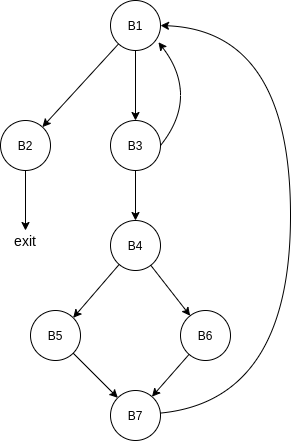
\includegraphics[scale=0.5]{cfg.png}
    \subsection*{(d)}
    B1 post-dominates nodes B3, B4, B5, B6, B7. \\
    B2 post-dominates every other node. \\
    B7 post-dominates B4, B5, B6.
\end{multicols}

\end{document}